\chapter{Experiments}
\label{cha:experiments}
\vspace{0.4 cm}

In this chapter, write the State of the art...

\section{Experimental Setup}
\label{sec:experimental_setup}
\vspace{0.2 cm}

In this section, a brief introduction to ... 

\vspace{0.1 cm}
\subsection{Pre-processing}
\label{sec:preprocessing}
\vspace{0.1 cm}

In this subsection, an overview of ...

\vspace{0.1 cm}
\subsection{Evaluation Metrics}
\label{sec:evaluation_metrics}
\vspace{0.1 cm}

In this subsection, ...

\section{Research Questions}
\label{sec:research_questions}
\vspace{0.2 cm}

In this section, we will discuss the research questions which are as follows:
\begin{itemize}
  \item RQ1: How effective the LLMs are to generate test Oracles?
  \item RQ2: How efficient the LLMs are to generate test Oracles?
\end{itemize}

\section{Results}
\label{sec:results}
\vspace{0.2 cm}

In this section, a brief introduction to ... 

\vspace{0.1 cm}
\subsection{RQ1: Effectiveness of LLMs}
\label{sec:results_rq1}
\vspace{0.1 cm}

In this subsection, an overview of ...




\begin{table}[H]
\centering

\begin{tabular}{| l | r | r | r | r | r | r |}
\hline
\multirow{2}{*}{\textbf{Class}} & \multirow{2}{*}{\textbf{EvoSuite}} & \multicolumn{5}{c|}{\textbf{EvoOracle}} \\ % Fix multicolumn formatting
\cline{3-7} % Add a horizontal line between the headers
 &  & \textbf{MPT-7B} & \textbf{Nous} & \textbf{Orca} & \textbf{Stable} & \textbf{WizardLM} \\
 &  &  & \textbf{hermes-13b} & \textbf{mini\_13B} & \textbf{Vicuna-13B} & \textbf{13B-V1.1} \\
\hline
\scriptsize\textsc{} &  &  &  &  &  &  \\
\scriptsize\textsc{BaseSettings} & 100 & 92.75 & 98.55 & 85.51 & 0 & 21.74 \\
\hline
\scriptsize\textsc{} &  &  &  &  &  &  \\
\scriptsize\textsc{CacheHandler} & 51.52 & 0 & 45.45 & 38.38 & 0 & 24.24 \\
\hline
\scriptsize\textsc{} &  &  &  &  &  &  \\
\scriptsize\textsc{NPMInstaller} & 46.49 & 6.14 & 19.3 & 2.05 & 6.14 & 6.14 \\
\hline
\scriptsize\textsc{} &  &  &  &  &  &  \\
\scriptsize\textsc{NodeInstaller} & 53.04 & 25.97 & 40.51 & 14.18 & 0 & 11.97 \\
\hline
\scriptsize\textsc{} &  &  &  &  &  &  \\
\scriptsize\textsc{Parallel} & 100 & 21.14 & 94.31 & 0 & 82.93 & 86.18 \\
\hline
\scriptsize\textsc{} &  &  &  &  &  &  \\
\scriptsize\textsc{PnpmInstaller} & 41.53 & 19.21 & 25.99 & 11.02 & 3.67 & 10.17 \\
\hline
\scriptsize\textsc{Properties} &  &  &  &  &  &  \\
\scriptsize\textsc{ProviderUtils} & 57.14 & 38.09 & 40.47 & 25 & 0 & 47.62 \\
\hline
\scriptsize\textsc{} &  &  &  &  &  &  \\
\scriptsize\textsc{ResolutionCache} & 18.92 & 18.92 & 18.92 & 6.31 & 18.92 & 18.92 \\
\hline
\scriptsize\textsc{SeekableByte} &  &  &  &  &  &  \\
\scriptsize\textsc{ArrayOutputStream} & 100 & 12.5 & 66.67 & 18.75 & 31.25 & 43.75 \\
\hline
\scriptsize\textsc{Zerocode} &  &  &  &  &  &  \\
\scriptsize\textsc{Correlationship} &  &  &  &  &  &  \\
\scriptsize\textsc{Logger} & 91.38 & 36.21 & 83.91 & 1.15 & 0 & 52.87 \\
\hline

\end{tabular}
\caption{Average Line Coverage by Class and Models.}
\label{tab:line_coverage}
\end{table}

\begin{table}[H]
\centering

\begin{tabular}{| l | r | r | r | r | r | r |}
\hline
\multirow{2}{*}{\textbf{Class}} & \multirow{2}{*}{\textbf{EvoSuite}} & \multicolumn{5}{c|}{\textbf{EvoOracle}} \\ % Fix multicolumn formatting
\cline{3-7} % Add a horizontal line between the headers
 &  & \textbf{MPT-7B} & \textbf{Nous} & \textbf{Orca} & \textbf{Stable} & \textbf{WizardLM} \\
 &  &  & \textbf{hermes-13b} & \textbf{mini\_13B} & \textbf{Vicuna-13B} & \textbf{13B-V1.1} \\
\hline
\scriptsize\textsc{} &  &  &  &  &  &  \\
\scriptsize\textsc{BaseSettings} & 53.33 & 13.33 & 37.78 & 20 & 0 & 2.22 \\
\hline
\scriptsize\textsc{} &  &  &  &  &  &  \\
\scriptsize\textsc{CacheHandler} & 27.78 & 0 & 0 & 0 & 0 & 0 \\
\hline
\scriptsize\textsc{} &  &  &  &  &  &  \\
\scriptsize\textsc{NPMInstaller} & 34.09 & 0 & 12.12 & 0 & 0 & 0 \\
\hline
\scriptsize\textsc{} &  &  &  &  &  &  \\
\scriptsize\textsc{NodeInstaller} & 56.9 & 27.59 & 45.98 & 12.07 & 0 & 12.07 \\
\hline
\scriptsize\textsc{} &  &  &  &  &  &  \\
\scriptsize\textsc{Parallel} & 100 & 7.69 & 60.26 & 0 & 33.33 & 51.28 \\
\hline
\scriptsize\textsc{} &  &  &  &  &  &  \\
\scriptsize\textsc{PnpmInstaller} & 29.27 & 8.94 & 14.63 & 0.00 & 1.63 & 4.07 \\
\hline
\scriptsize\textsc{Properties} &  &  &  &  &  &  \\
\scriptsize\textsc{ProviderUtils} & 26.67 & 15.55 & 11.11 & 6.67 & 0 & 8.89 \\
\hline
\scriptsize\textsc{SeekableByte} &  &  &  &  &  &  \\
\scriptsize\textsc{ArrayOutputStream} & 93.75 & 0 & 60.42 & 14.58 & 31.25 & 25 \\
\hline
\scriptsize\textsc{Zerocode} &  &  &  &  &  &  \\
\scriptsize\textsc{Correlationship} &  &  &  &  &  &  \\
\scriptsize\textsc{Logger} & 52.38 & 6.35 & 25.4 & 1.59 & 0 & 28.57 \\
\hline

\end{tabular}
\caption{Average Mutation Coverage by Class and Models.}
\label{tab:mutation_coverage}
\end{table}

\begin{table}[H]
\centering

\begin{tabular}{| l | r | r | r | r | r | r |}
\hline
\multirow{2}{*}{\textbf{Class}} & \multirow{2}{*}{\textbf{EvoSuite}} & \multicolumn{5}{c|}{\textbf{EvoOracle}} \\ % Fix multicolumn formatting
\cline{3-7} % Add a horizontal line between the headers
 &  & \textbf{MPT-7B} & \textbf{Nous} & \textbf{Orca} & \textbf{Stable} & \textbf{WizardLM} \\
 &  &  & \textbf{hermes-13b} & \textbf{mini\_13B} & \textbf{Vicuna-13B} & \textbf{13B-V1.1} \\
\hline
\scriptsize\textsc{} &  &  &  &  &  &  \\
\scriptsize\textsc{BaseSettings} & 53.33 & 13.33 & 37.78 & 22.96 & 0 & 3.33 \\
\hline
\scriptsize\textsc{} &  &  &  &  &  &  \\
\scriptsize\textsc{CacheHandler} & 71.43 & 0 & 0 & 0 & 0 & 0 \\
\hline
\scriptsize\textsc{} &  &  &  &  &  &  \\
\scriptsize\textsc{NPMInstaller} & 71.43 & 0 & 52.38 & 0 & 0 & 0 \\
\hline
\scriptsize\textsc{} &  &  &  &  &  &  \\
\scriptsize\textsc{NodeInstaller} & 100 & 62.58 & 100 & 40.1 & 0 & 30.43 \\
\hline
\scriptsize\textsc{} &  &  &  &  &  &  \\
\scriptsize\textsc{Parallel} & 100 & 8.7 & 62.5 & 0 & 35.41 & 54.51 \\
\hline
\scriptsize\textsc{} &  &  &  &  &  &  \\
\scriptsize\textsc{PnpmInstaller} & 70.59 & 22.92 & 40.00 & 0.00 & 33.33 & 38.33 \\
\hline
\scriptsize\textsc{Properties} &  &  &  &  &  &  \\
\scriptsize\textsc{ProviderUtils} & 66.67 & 50 & 27.78 & 33.33 & 0 & 25 \\
\hline
\scriptsize\textsc{SeekableByte} &  &  &  &  &  &  \\
\scriptsize\textsc{ArrayOutputStream} & 93.75 & 0 & 73.68 & 44.44 & 100 & 58.59 \\
\hline
\scriptsize\textsc{Zerocode} &  &  &  &  &  &  \\
\scriptsize\textsc{Correlationship} &  &  &  &  &  &  \\
\scriptsize\textsc{Logger} & 55 & 16.93 & 31.56 & 16.67 & 0 & 45.63 \\
\hline

\end{tabular}
\caption{Average Test Strength by Class and Models.}
\label{tab:test_strength}
\end{table}

\begin{figure}[H]
\centering
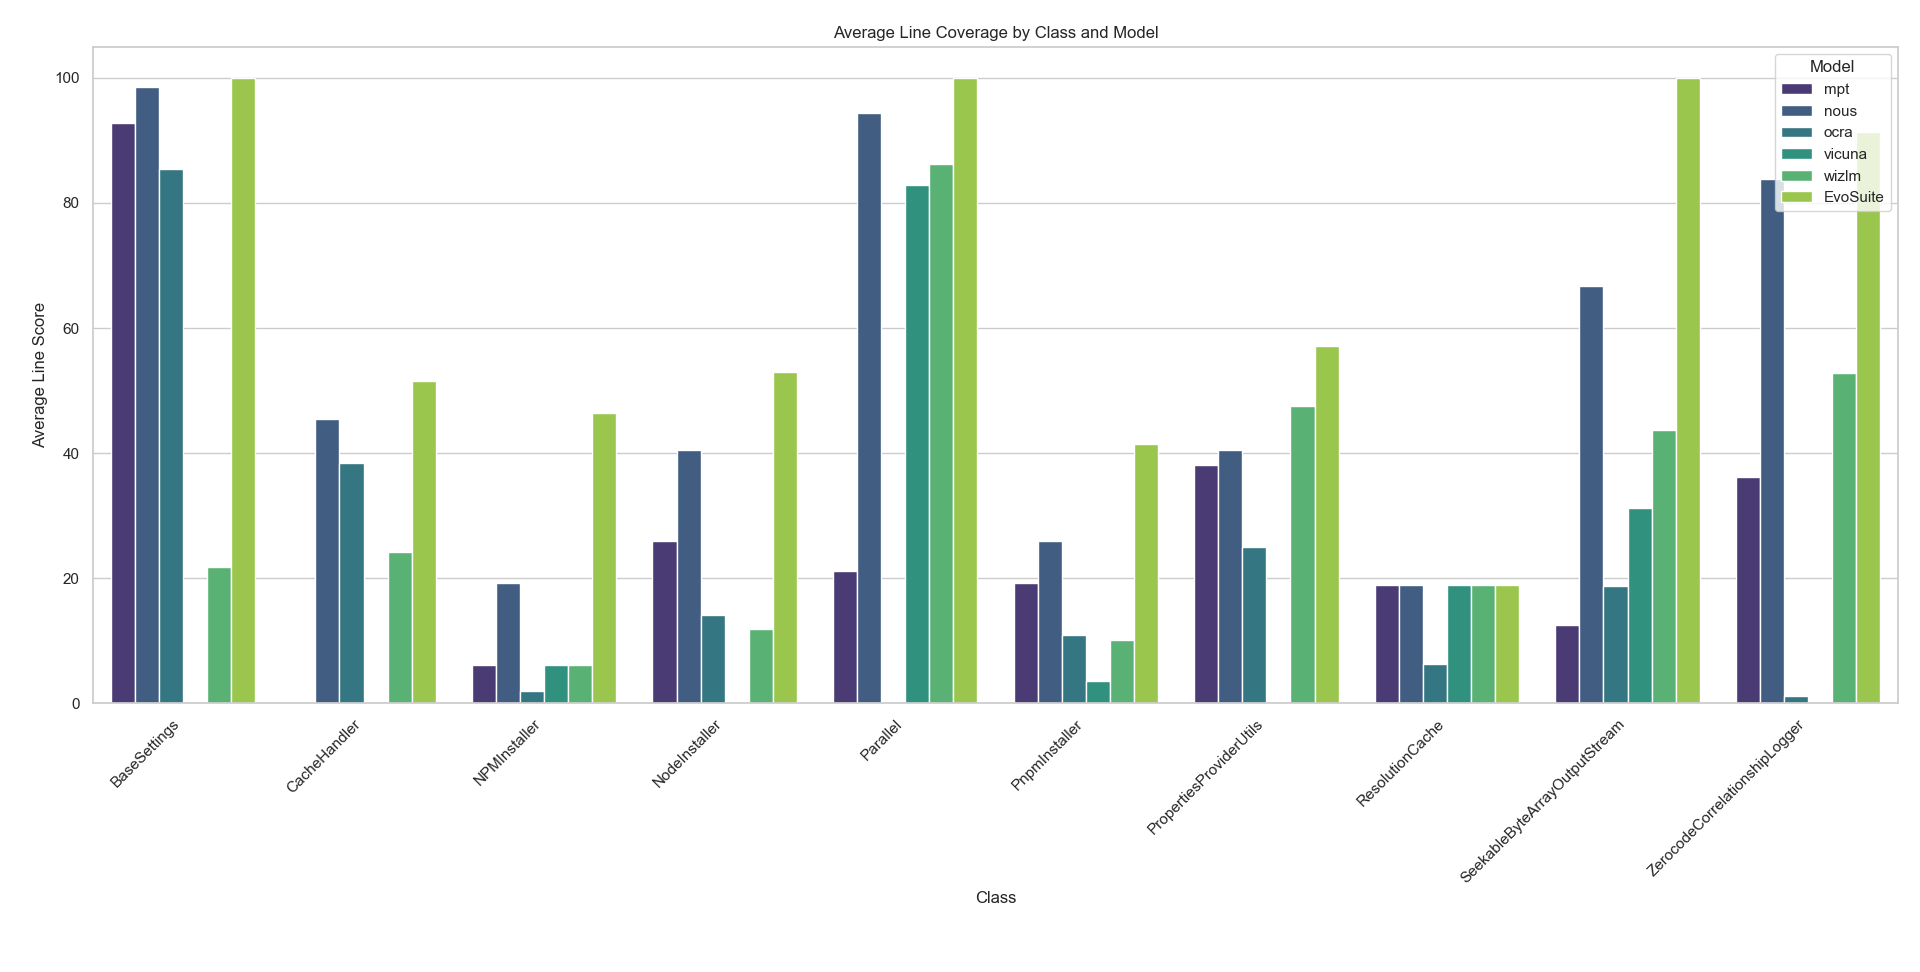
\includegraphics[width=1\textwidth]{images/line_coverage.png}
\caption{Average Line Coverage by Class and Models}
\label{fig:line_coverage}
\end{figure}

\begin{figure}[H]
\centering
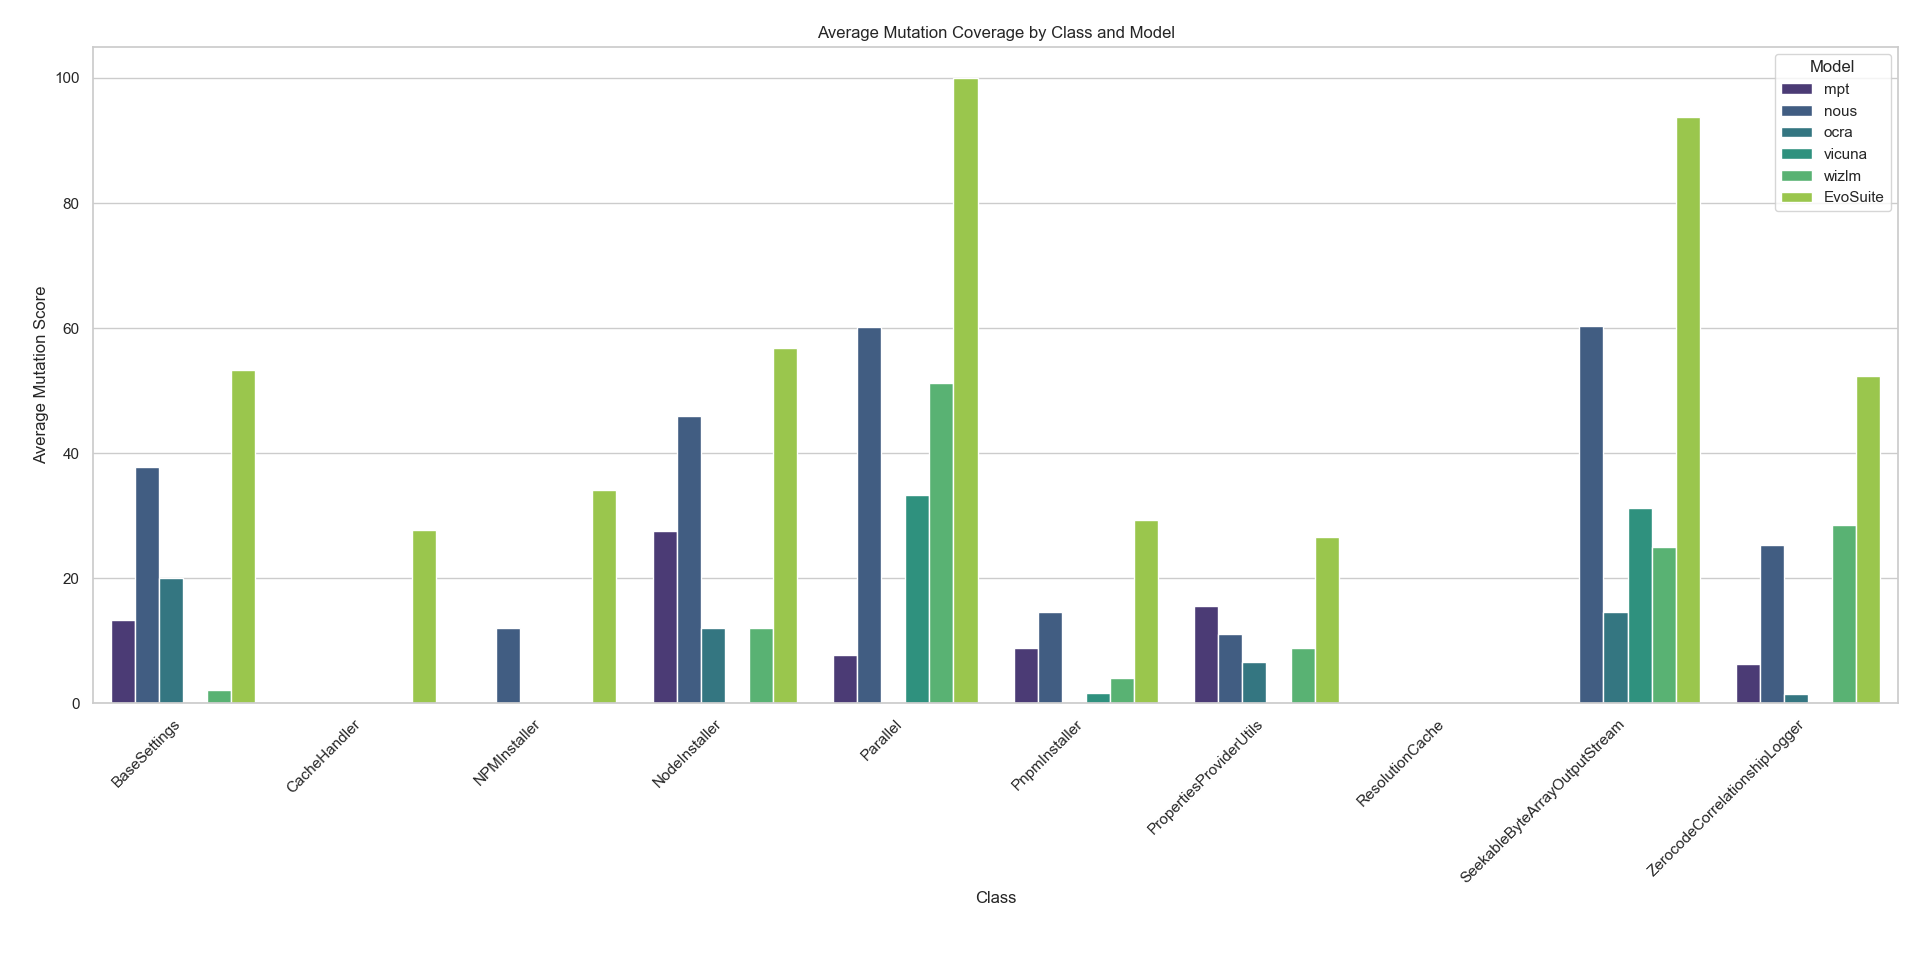
\includegraphics[width=1\textwidth]{images/mutation_coverage.png}
\caption{Average Mutation Coverage by Class and Models}
\label{fig:mutation_coverage}
\end{figure}

\begin{figure}[H]
\centering
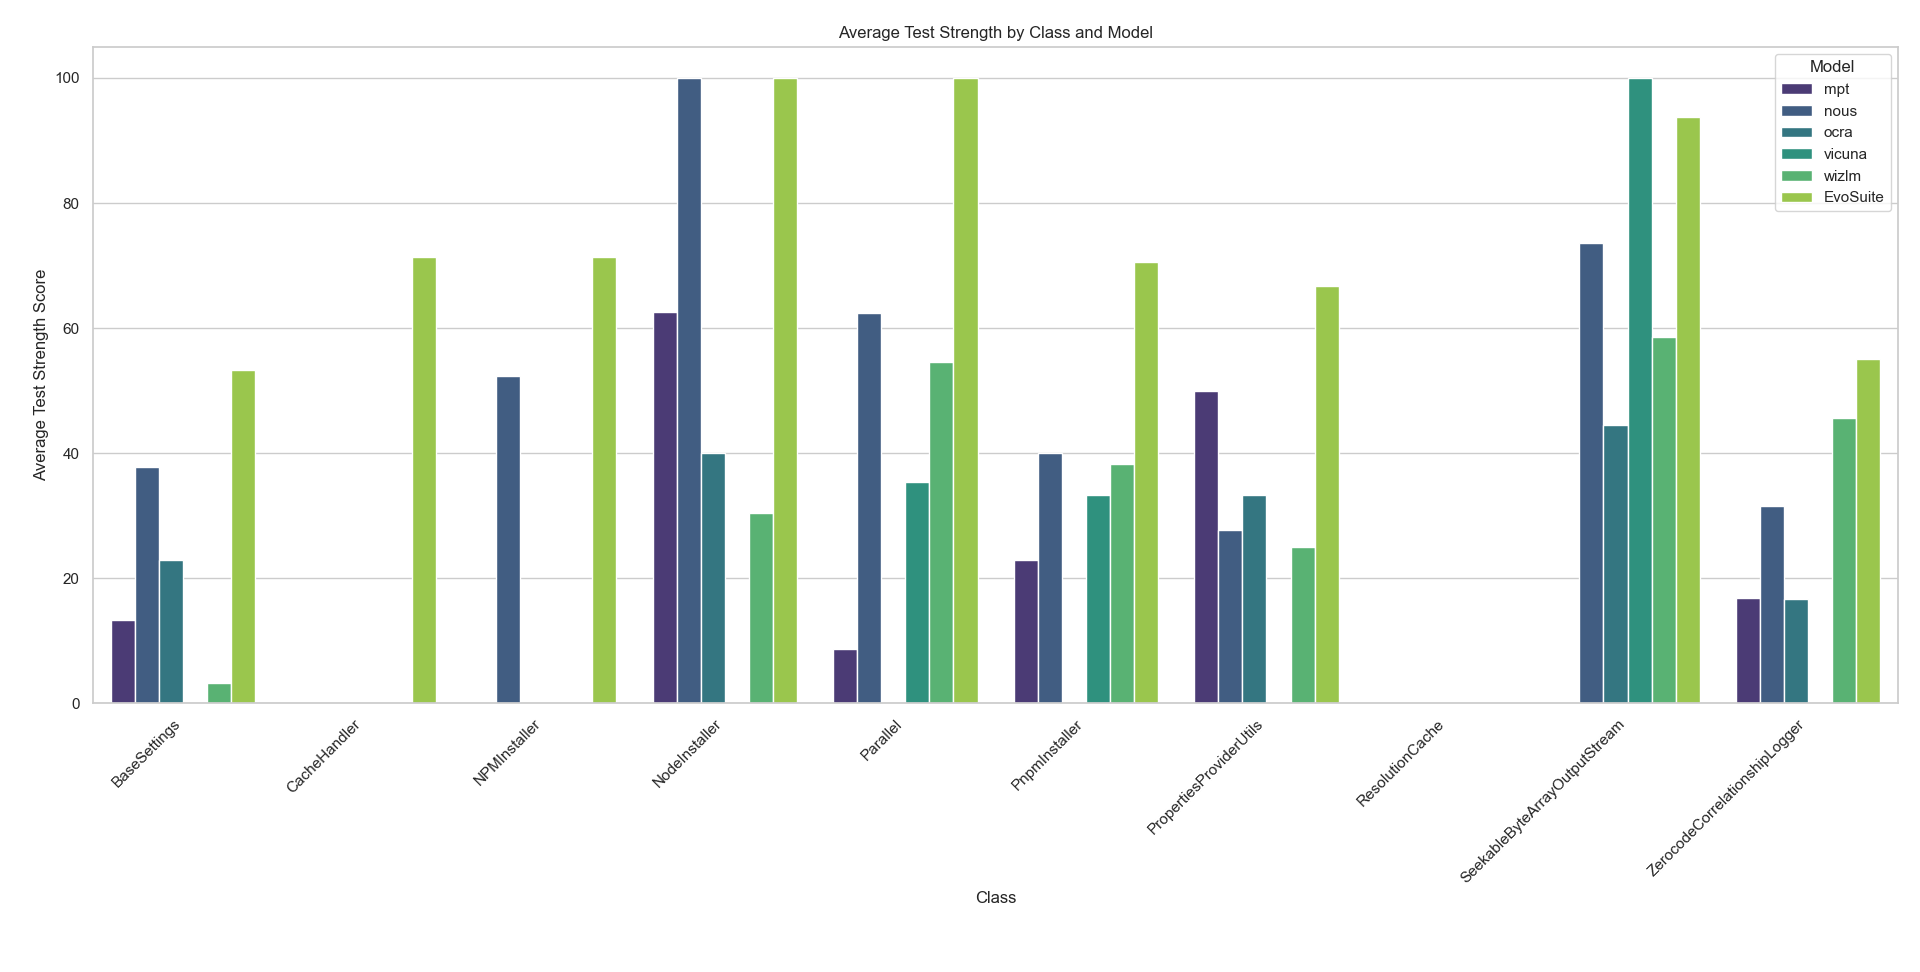
\includegraphics[width=1\textwidth]{images/test_strength.png}
\caption{Average Test Strength by Class and Models}
\label{fig:test_strength}
\end{figure}

\vspace{0.1 cm}
\subsection{RQ2: Efficiency of LLMs}
\label{sec:results_rq2}
\vspace{0.1 cm}

In this subsection, an overview of ...

\section{Threats to Validity}
\label{sec:t2v}
\vspace{0.2 cm}

In this section, we will discuss many things. There will also be footnotes\footnote{ \url{https://www.footnote.com/} }. This is how we cite\cite{Nguyen2019} provided a case study

\section{Discussion and Future Work}
\label{sec:discussion}
\vspace{0.2 cm}

In this section, a brief introduction to ... 

% \vspace{0.1 cm}
% \subsection{Subsection}
% \label{sec:transformers}
% \vspace{0.1 cm}

% In this subsection, an overview of ...

% \vspace{0.1 cm}
% \subsection{Another Subsection}
% \label{sec:automl}
% \vspace{0.1 cm}

% In this subsection, ...